\documentclass[a4paper,12pt]{article}

\usepackage[margin=2.5cm]{geometry}
\usepackage{fix-cm}
\usepackage{indentfirst}
\usepackage{graphicx}
\usepackage{fancyhdr}
\usepackage{setspace}
\usepackage{enumerate}
%\usepackage{hyperref}
\usepackage{color}
\usepackage{colortbl}
\usepackage[small]{caption}
\usepackage{enumitem}
\usepackage{amsmath}
\usepackage{mathtools}
\usepackage{amsfonts}
\usepackage{multirow}

\DeclarePairedDelimiter{\ceil}{\lceil}{\rceil}

\linespread{1.2}
\setlength{\parskip}{5pt}
\setlength{\parindent}{0.5cm}

%Header and Footer
\fancyhead{} \fancyhead[LO,RE]{\scriptsize\sc\leftmark}
\fancyfoot[l]{ \scriptsize \textit{UCI, Spring 2013}}
\fancyfoot[R]{ \scriptsize \textit{CS 222 - Project Report - Part 02}}



\begin{document}
\begin{titlepage}

\noindent
\begin{minipage}{0.8\textwidth}
\begin{flushleft}
\noindent
\begin{large}
\textbf{University of California Irvine}
\end{large}

\noindent
\begin{small}
\textbf{Donald Bren School of Information and Computer Sciences}\\
\end{small}

\noindent
\begin{small}
\textbf{Department of Computer Science}\\
\end{small}
\end{flushleft}
\end{minipage}
\begin{minipage}{0.2\textwidth}
\begin{flushright}

\includegraphics[scale=0.25]{Figures/uci_logo.png}
\end{flushright}
\end{minipage}\\



\begin{center}
\begin{large}
CS 222 - Principles of Data Management
\end{large}
\end{center}

\vspace{1.5cm}

\begin{center}
\begin{LARGE}
\textsc{Project Report - Part 02}
\end{LARGE}
\end{center}

\vspace{2.5cm}

\begin{figure}[h]
\centering
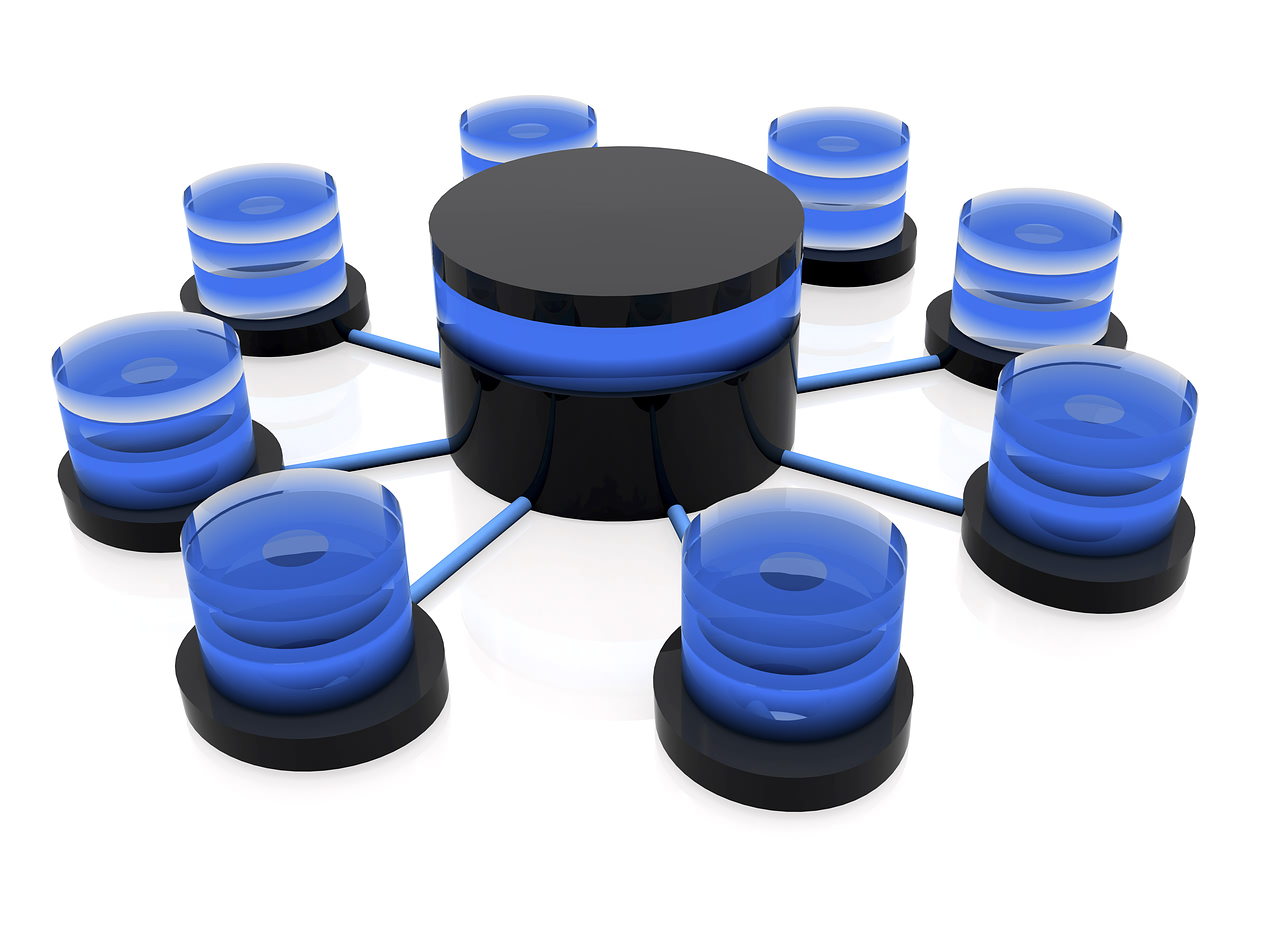
\includegraphics[scale=1]{Figures/database.png}
\end{figure}

\vspace{2.5cm}

\begin{center}
\begin{Large}
\textbf{Sky Faber} \quad\quad \textbf{Ekin Oguz} \quad\quad \textbf{Cesar Ghali}
\end{Large}
\end{center}
\end{titlepage}


\pagenumbering{roman}
\setcounter{page}{1}


\setcounter{tocdepth}{3}






\newpage



\pagestyle{fancy}
\pagenumbering{arabic}
\setcounter{page}{1}

\section{Catalog}
The database catalog contains two self-describing tables, tables and columns. Tables table contains information (table name, file location, file type, version) about each table created in the database. The version indicates the latest version of the table in the database. The columns table contains information about each column in all the tables in the database. The information stored is column name, table name, position, type, length, nullable, version. The version contains what version the table is in. Whenever an attribute is added or dropped from the table, the version field is increased. In addition, the version of each record is stored along the record in the database. The idea behind versioning is that when a table is altered, all old records are untouched. When a tuple is read or the table is scanned, all old versions will be reformatted in the most recent version of the table.

\section{Record Format}
Each record with $n$ fields is formatted as follows:
\begin{itemize}
\item The first byte is a boolean specifying whether this record is a forward pointer or not.
\item The second byte is the version of this record (more about this later).
\item $n + 1$ offset pointers (each one is two bytes). Each one points to the beginning of the corresponding field and the last offset pointer points to the end of the record.
\item After the fields directory, all $n$ fields are concatenated.
\end{itemize}

Using this format accessing any filed takes $O(1)$ operation. It is also not necessary to store the length of the field. Instead, it can be calculate on the fly with $P(1)$ operations. The offset of the first field is read, then the end offset of the field is read (value of first offset - 2) which indicates the length of the field.

\section{Page Format}
Pages in the database contain records of variable length. All records are packed to the begin of the page. The last two bytes of the page contains the offset of the beginning of the empty space on page. Right before these two bytes, the record directory is located. This directory contains in its first two bytes the number of records in the directory. The rest of the directory contains two bytes offset for the beginning of the records on the page.

The first page contains information about the free spaces on each page of the file. The first two bytes of the page contains the number of pages on the file. Then each two bytes contains the amount of free space on each page.

\subsection{Operations on records}
\begin{enumerate}
\item Record Deletion: when a record is deleted, its slot in the records directory is assigned the value \texttt{0xFFFF} rending this slot to be empty. In addition, when a record is deleted, its physical location on the page is kept empty and the free space on the first page is updated.
\item Record Addition: when a record is added, the directory is scanned for the first empty slot (marked with \texttt{0xFFFF}) to be used. If such a slot could not be found, a new slot is added to the end of directory and the number if records is increased. Note that the offset where the record is stored on the page is obtained from the last two bytes of the page (the empty space offset). Also the free space on the first page is also updated to reflect the addition of a new record to this page.\\
The addition algorithm consults the first page of the file looking for a page with free space. When such a page is found and the record cannot fit at the end of the page (starting where the free space pointer points) the page is reorganized but without changing the slot numbers. If no pages have free space, a new page is added to the file.
\item Record update: updating a record is basically deleting that record and add it again but in the same page and at the same slot number. If there record cannot fit on the page, a forward pointer is created. The forward pointer contains the alien page number and the slot number of this record. Note that when a record is updated, it should be located on the same page and at the same slot number as before, so a forward pointer is updated to point to the place where the record is stored in case that page was full. This whole operation is transparent for any upper layer.
\end{enumerate}

\section{Altering the database}
The columns table of the catalog contains information about all the columns in each table in the database. When a new column is added to a table, the latest (in terms of version) catalog information about this table is read, then reinserted with a new version number. When a column is deleted, all the old versioned information is reinserted with a new version but without the deleted column. Note that reading records or scanning a table will take care of converting all the filed to the latest version on the fly. Records are not reformatted and stored in the file unless the whole table is reorganized.

\section{Table Reorganization}
When a table version reaches a certain predefined threshold, e.g. 10, the whole table is reorganized. At this point, all records are read, converted to the latest version and stored in the file without changing their RIDs. If a record cannot fit on the page that it was located in, a forward pointer is used. Unfortunately, this feature is not implemented.
 

\end{document}
